\documentclass[14pt]{beamer}

\usepackage[absolute,overlay]{textpos}

%
% STYLE
%
\AtBeginSection{%
  \begin{frame}
    \sectionpage
  \end{frame}
}

\usepackage[inline]{enumitem}

\setlist*[itemize]{
    label={-},
    font={},
    leftmargin=*
}


\setbeamertemplate{section page}{
  \begin{center}
    
\includegraphics[width=6cm]{img/logo.png}

    \vspace{1cm}
    \usebeamerfont{title}\insertsectionhead\par%
  \end{center}
}

\setbeamertemplate{navigation symbols}{}

\setbeamertemplate{footline}[frame number]

\setbeamerfont{title}{size=\large}

\makeatletter
\setbeamertemplate{title page}{
  \vbox{}
  \vfill
  \begingroup
    \centering
    
\includegraphics[width=6cm]{img/logo.png}
    \vskip2em\par
    \begin{beamercolorbox}[sep=8pt,center]{title}
      \usebeamerfont{title}\inserttitle\par%
    \end{beamercolorbox}%
    \vskip2em\par
    \begin{minipage}{0.4\textwidth}
      
\includegraphics[width=4cm]{img/capitole_du_libre_logo.png}
    \end{minipage}
    \begin{minipage}{0.5\textwidth}
      \begin{beamercolorbox}[sep=8pt,center]{author}
        \usebeamerfont{author}\insertauthor
      \end{beamercolorbox}
      \begin{beamercolorbox}[sep=8pt,center]{date}
        \usebeamerfont{date}\insertdate
      \end{beamercolorbox}
    \end{minipage}
    {\usebeamercolor[fg]{titlegraphic}\inserttitlegraphic\par}
  \endgroup
  \vfill
}
\makeatother

%
% COLORS
%
\usepackage[]{xcolor}

\definecolor{background}{HTML}{3f3c35}
\definecolor{normal-text}{HTML}{fefdf9}
\definecolor{accent}{HTML}{f77f00}

\setbeamercolor{background canvas}{bg=background}
\setbeamercolor{normal text}{fg=normal-text}
\setbeamercolor{titlelike}{fg=normal-text}

\renewcommand{\emph}[1]{\textcolor{accent}{#1}}

%
% FONTS
%
\usepackage{fontspec}
\setmainfont{monofur}
\setsansfont{monofur}
\setmonofont{monofur}



\title{Une plateforme web Open Source de partage et d'échange collaboratif autour du travail du bois }
\author{Etienne Monier}
\date{19 novembre 2023}

\begin{document}

\begin{frame}[plain]
  \titlepage
\end{frame}

\section{Un réseau social solidaire ?}

\begin{frame}
\frametitle{Un réseau social ?}

\begin{itemize}
  \item Projet de plateforme \emph{non commerciale} initié en 2013 par Boris Beaulant
  \item Espace d'\emph{échange} numérique
  \item Passion commune : \emph{le travail du bois}
  \item Communauté ouverte
\end{itemize}

\bigskip

\begin{minipage}{0.45\textwidth}
  {\small
  39\;000 inscrits

  2\;000\;000 visiteurs/an

  21\;400 créations
  }
\end{minipage}
\begin{minipage}{0.45\textwidth}
  \begin{figure}
    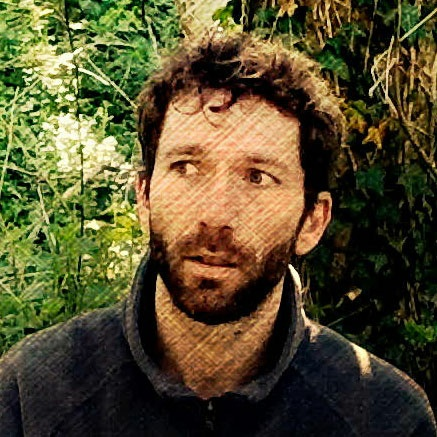
\includegraphics[width=2cm]{img/boris.jpg}
    {\center\small Boris Beaulant}
  \end{figure}
\end{minipage}
\end{frame}

\begin{frame}
\frametitle{Un réseau social \emph{solidaire} ?}

\begin{itemize}
  \item L'utilisateur \emph{n'est pas} le produit
  \item Contribution au \emph{Bien Commun}
  \item Communauté \emph{actrice} de sa plateforme
  \item Plateforme \emph{Open Source}
  \item Contenus publiés sous \emph{Creative Commons}
\end{itemize}
\end{frame}

\begin{frame}
  \begin{center}
    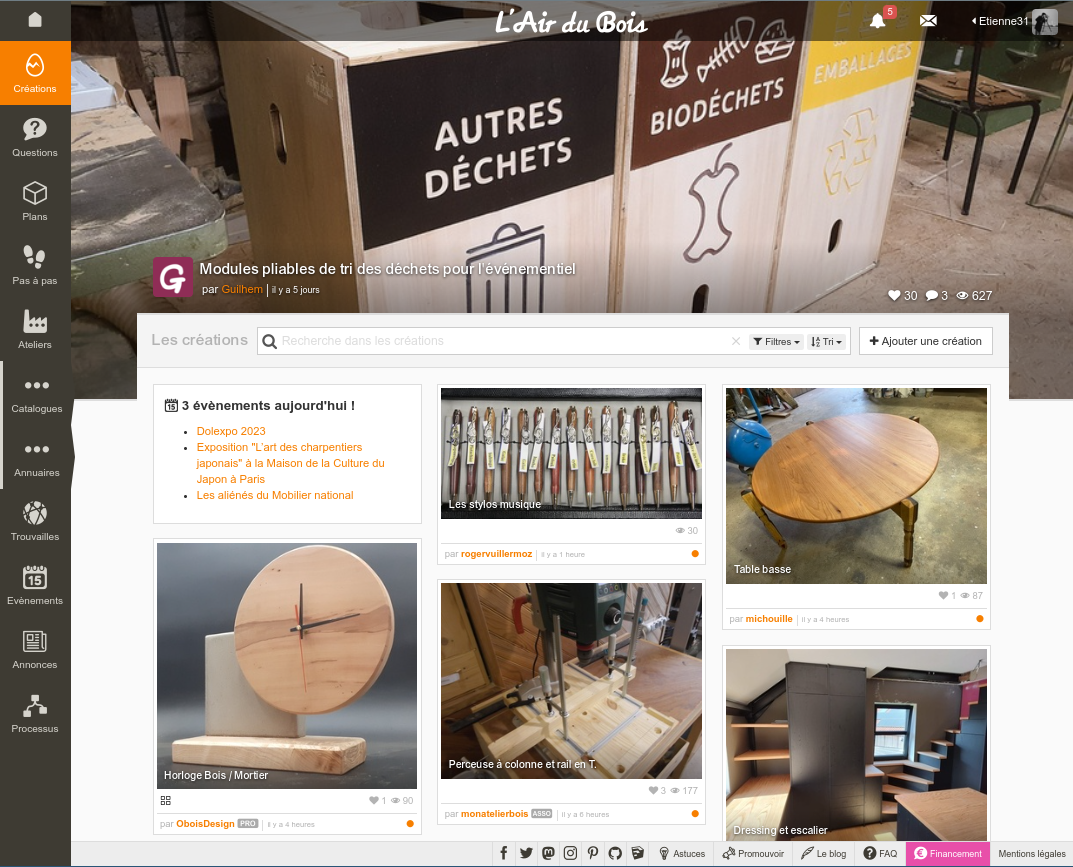
\includegraphics[width=\framewidth]{img/home.png}
  \end{center}
\end{frame}

\begin{frame}
  \begin{textblock*}{8cm}(0.5cm,0.5cm)
    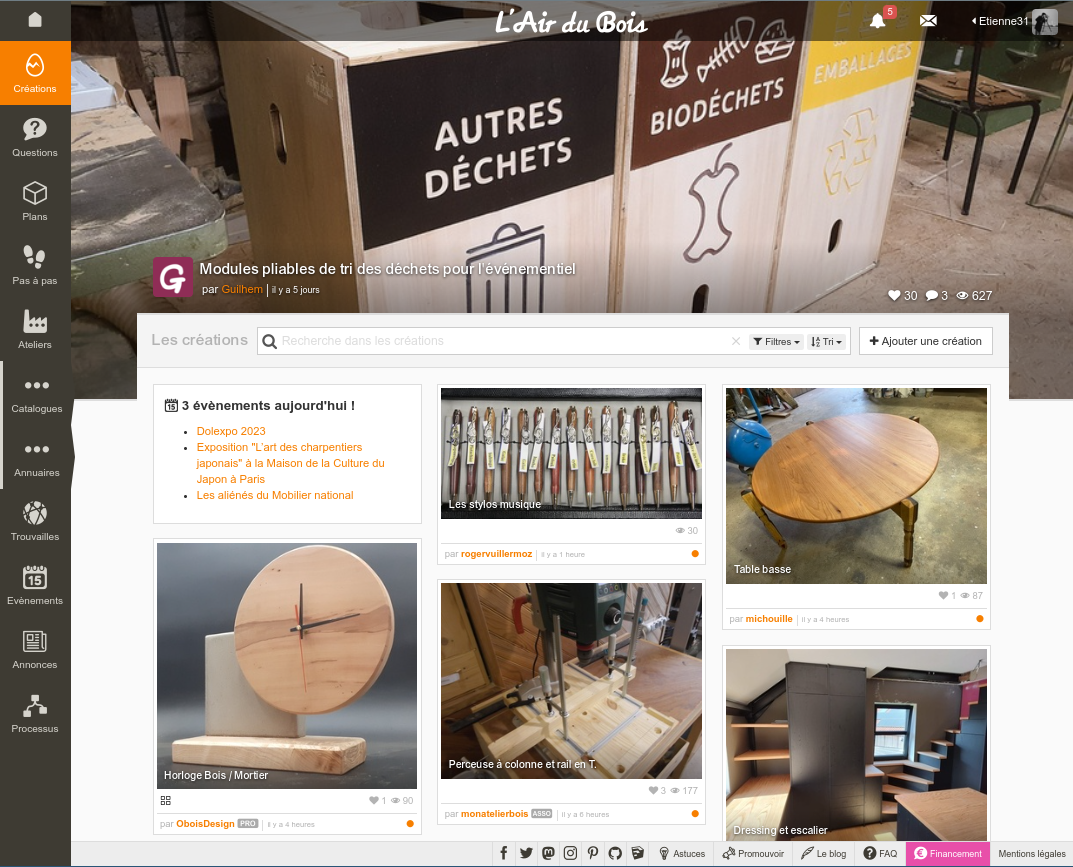
\includegraphics[width=8cm]{img/home.png}
    \end{textblock*}
  \begin{textblock*}{8cm}(4cm,2.5cm)
    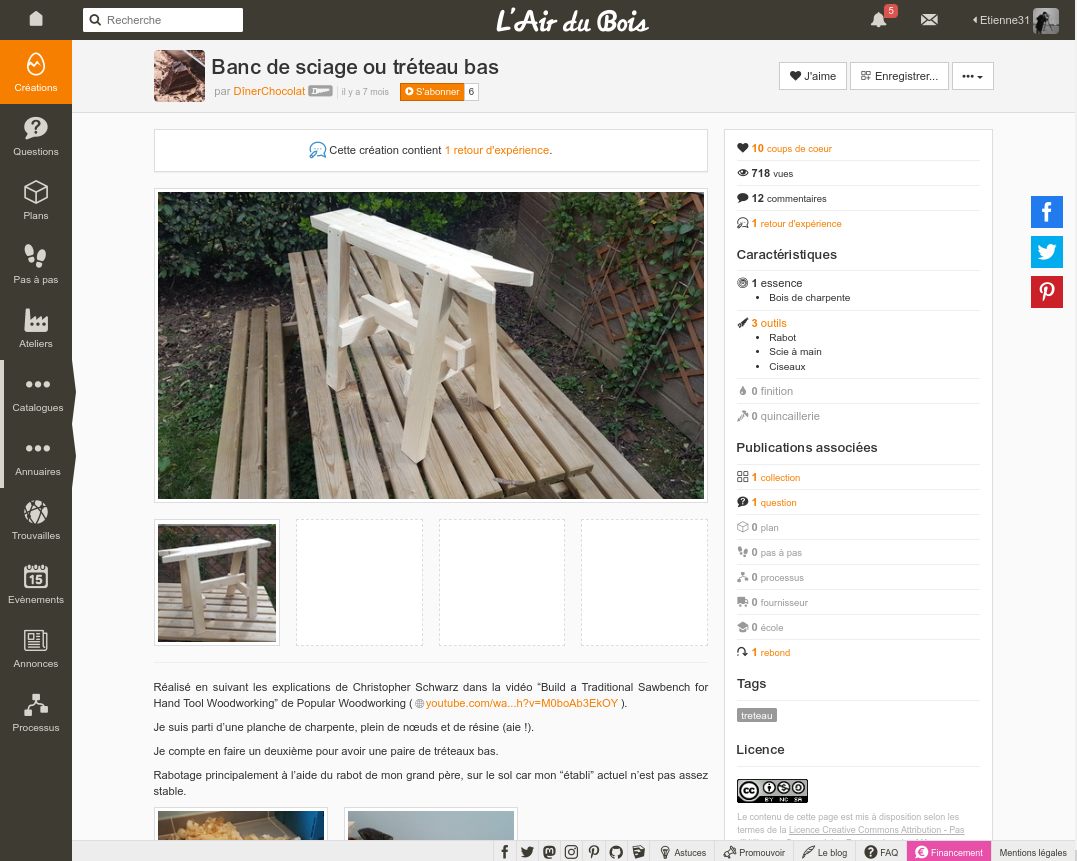
\includegraphics[width=8cm]{img/creation.png}
    \end{textblock*}

\end{frame}


\section{Pourquoi ?}

\begin{frame}
  \frametitle{Pourquoi ?}

  \begin{itemize}
    \item Pomouvoir le \emph{faire}
    \item Pomouvoir l'\emph{Open Source} dans l'artisanat
    \item Créer des outils adaptés à un domaine
    \smallskip
    {\small\begin{itemize}
      \item Annuaire collaboratif de \emph{fournisseur} et d'\emph{écoles}
      \item Xylothèque
      \item Outils d'organisation de production artisanale
    \end{itemize}}
    \smallskip
    \item Découvrir, Fabriquer, Partager
  \end{itemize}
\end{frame}

\begin{frame}
    \begin{center}
      \makebox[\textwidth][c]{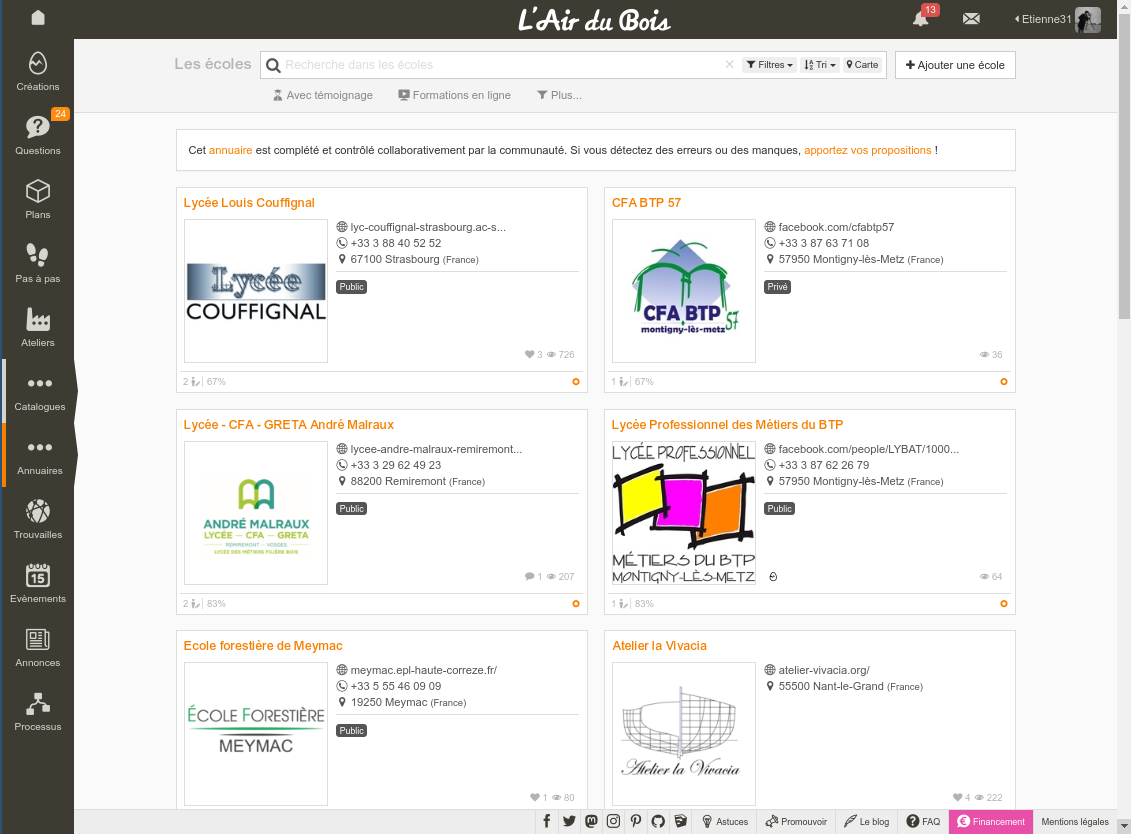
\includegraphics[width=11.5cm]{img/ecoles.png}}
    \end{center}
\end{frame}

\begin{frame}
  \begin{center}
    \makebox[\textwidth][c]{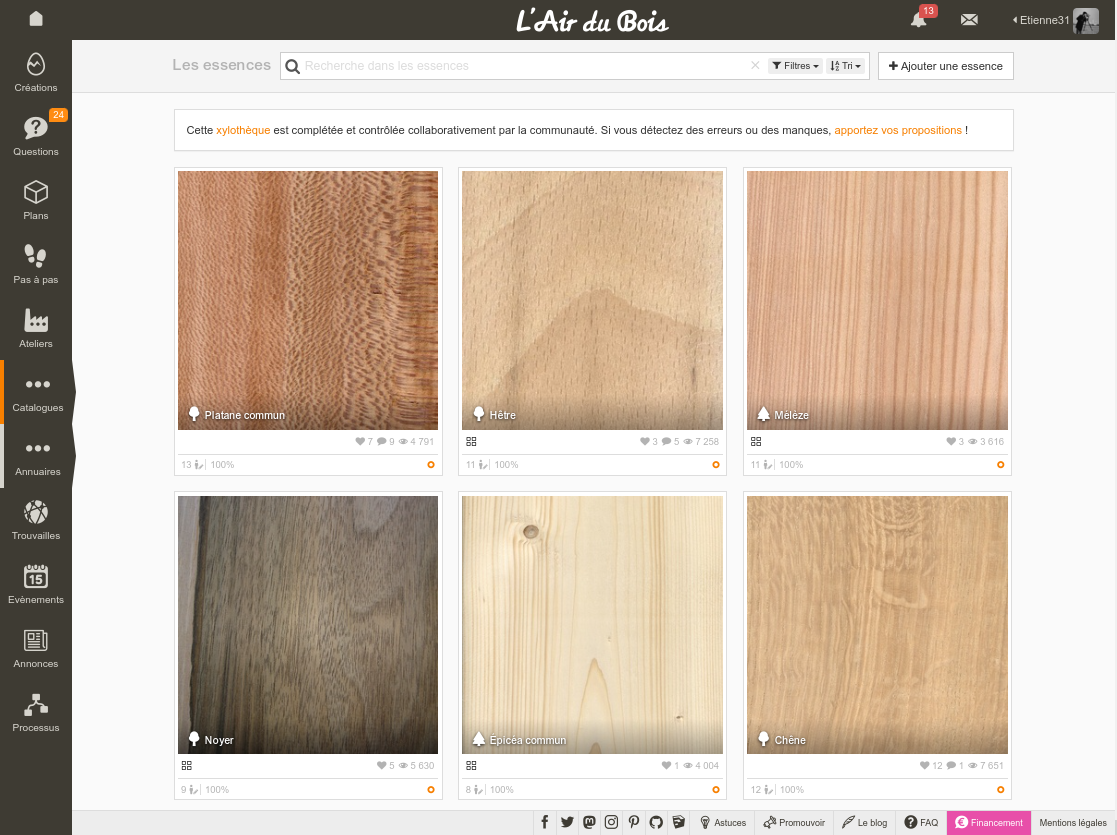
\includegraphics[width=11.5cm]{img/xylotheque.png}}
  \end{center}
\end{frame}

\begin{frame}
  \begin{center}
    \makebox[\textwidth][c]{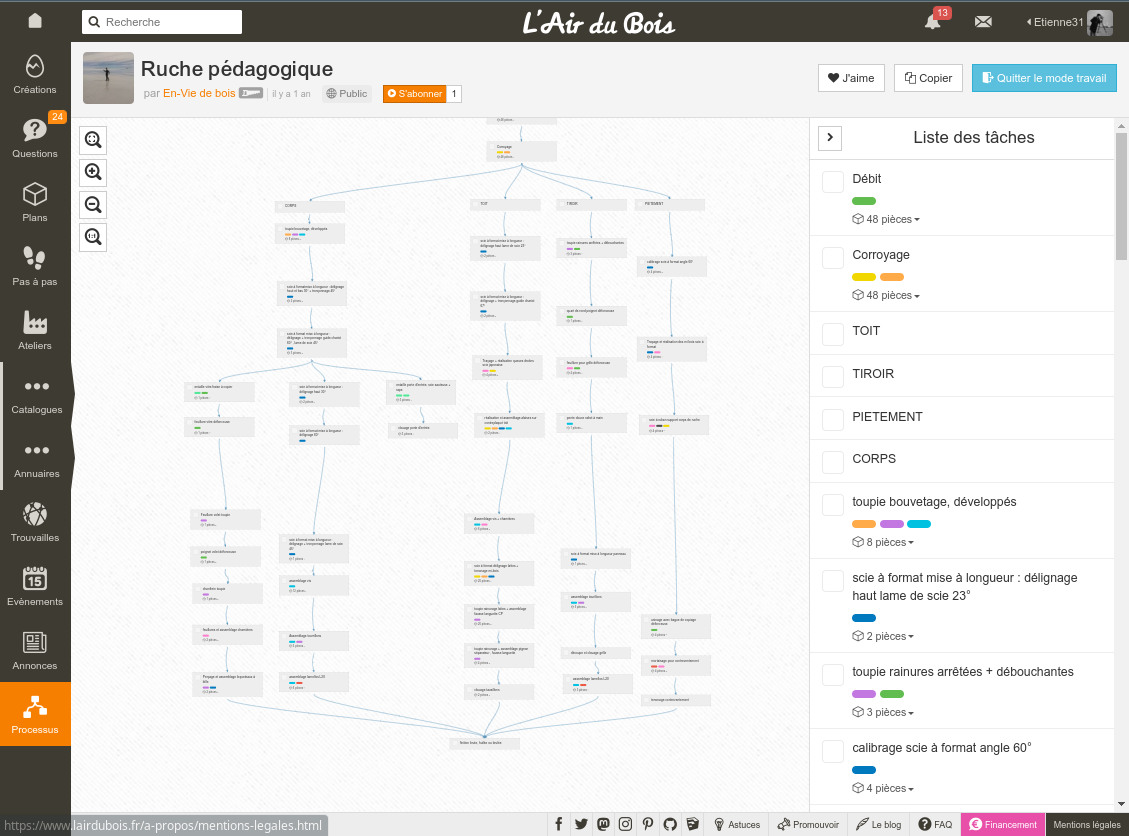
\includegraphics[width=11.5cm]{img/processus.png}}
  \end{center}
\end{frame}





\section{Les utilisateurs}

\begin{frame}
  \frametitle{Pour qui ?}

  \begin{itemize}
    \item Les PROs
    \item Les Amateurs
    \item Bref \dots \emph{tous} les amoureux du bois
  \end{itemize}
\end{frame}

\begin{frame}
  \frametitle{Faire rencontrer les utilisateurs}

  \begin{itemize}
    \item Rassemblement par \emph{collectifs}
    \item Rencontres autours de projets
    {\small\begin{itemize}
      \item \emph{salons} (Epinal, Maker Faire)
      \item \emph{projets} personels (zelo voyage)
    \end{itemize}}
    \item Pas de rassemblement national
  \end{itemize}
\end{frame}


\begin{frame}
  \begin{textblock*}{8cm}(0.5cm,0.5cm)
    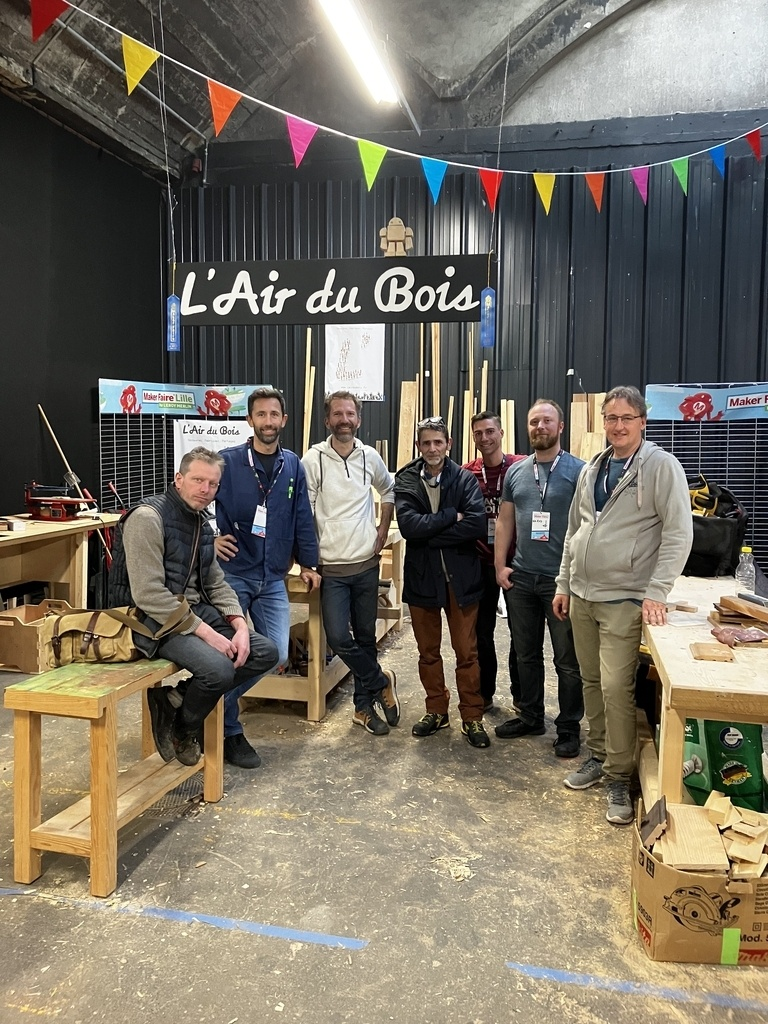
\includegraphics[width=5cm]{img/maker-lille-2022.jpg}
    \end{textblock*}
  \begin{textblock*}{8cm}(6cm,2.5cm)
    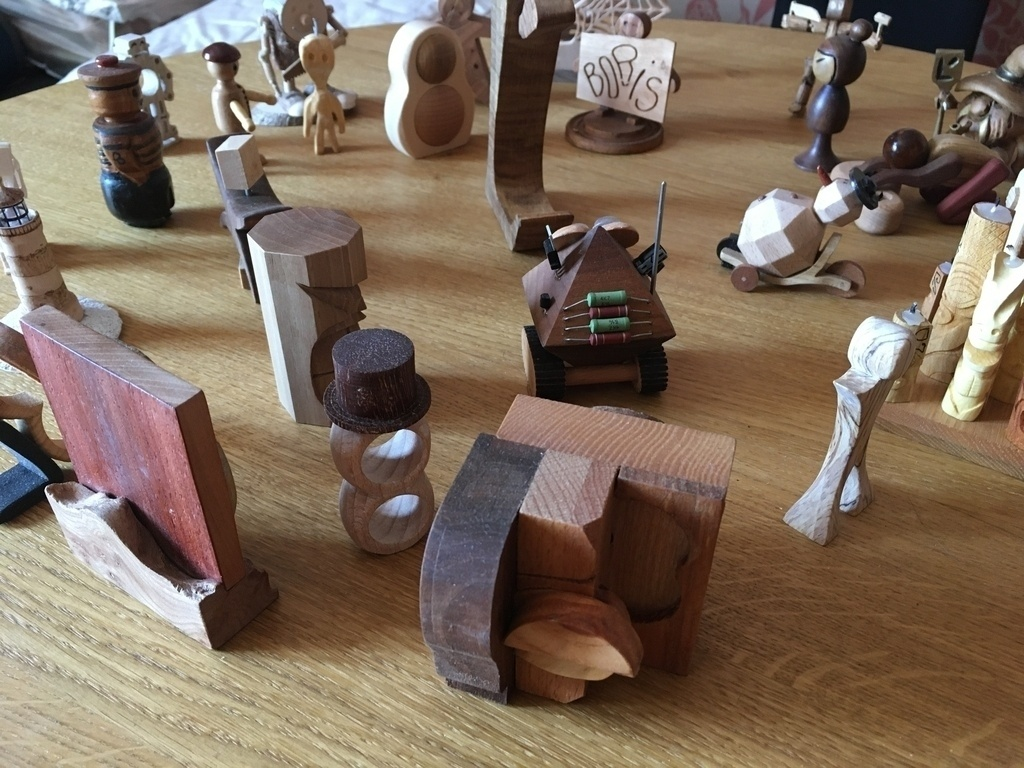
\includegraphics[width=6.5cm]{img/projet-8-ans.jpg}
    \end{textblock*}

\end{frame}


\section{Qu'est ce qu'on y partage ?}

\begin{frame}
  \frametitle{Qu'est ce qu'on y partage ?}

  \begin{itemize}
    \item Des projets (créations, plans, pas-à-pas)
    \item Des questionnements
    \item De l'expérience
    \item Du savoir (cours, catalogues, \dots)
    \item \dots
  \end{itemize}

  \quad
  \begin{center}
    \emph{Démo !}
  \end{center}
\end{frame}

\section{Comment ?}

\begin{frame}
  \frametitle{Comment ?}

  \begin{itemize}
    \item Pas de structure administrative
    \item \emph{Auto-financement} (dons)
    \item Une monnaie alternative : \emph{le Temps}
    \item Chacun contribue à sa hauteur
  \end{itemize}
\end{frame}

\section{Opencutlist}

\begin{frame}
  \frametitle{Opencutlist}

  \begin{itemize}
    \item projet \emph{Open Source} lancé en 2016
    \item aide à la CAO dans \emph{Sketchup}
    \item maintenu par la communauté l'air du bois
    \item financement participatif
    \item documentation et chaîne YouTube
  \end{itemize}

  \bigskip

  Un nouveau-venu récent : \emph{lairdubois-clippy}
\end{frame}

\begin{frame}
  \frametitle{Opencutlist: fonctionalitées}

  Permet de créer
  \begin{itemize}
    \item des fiches de débit
    \item des calepinages de découpe
    \item des étiquettes
    \item des estimations de \emph{coûts} et de poids
    \item des vues explosées
  \end{itemize}

\end{frame}

\begin{frame}
  \begin{center}
    \makebox[\textwidth][c]{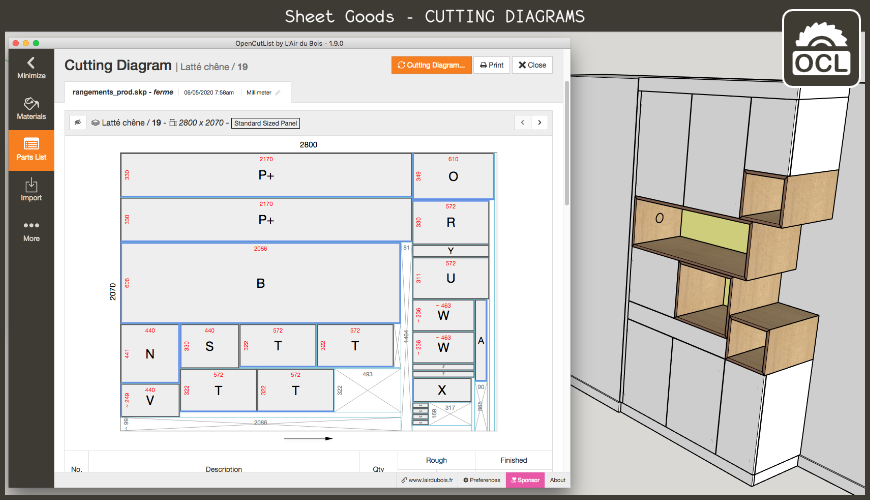
\includegraphics[width=11.5cm]{img/opencutlist.png}}
  \end{center}
\end{frame}


\begin{frame}
  \begin{center}
    
\includegraphics[width=6cm]{img/logo.png}

    www.lairdubois.fr

    \vspace{1cm}
    {\Large Merci !}
  \end{center}

  \begin{textblock*}{10cm}(0.5cm,7cm)
    
\includegraphics[width=3cm]{img/capitole_du_libre_logo.png}

    {\small Etienne Monier - 19 nov. 2023}
    \end{textblock*}

\end{frame}

\end{document}